\documentclass{article}

\usepackage{amsmath, amssymb}
\usepackage{xcolor}
\usepackage{caption, subcaption}
\usepackage{graphicx}
\usepackage{bm}             % For bold math symbols
\usepackage{soul}
\usepackage{outlines}   % For multilevel lists using the outline environment
\usepackage{tikz}
\usetikzlibrary{arrows.meta, positioning}


\usepackage{natbib}
\bibliographystyle{plainnat}

\usepackage{hyperref}   % For the \url{} command


\newcommand{\bG}{\mathbb{G}}
\newcommand{\bF}{\mathbb{F}}
\newcommand{\bP}{\mathbb{P}}
\newcommand{\bE}{\mathbb{E}}
\newcommand{\bV}{\mathbb{V}}

\newcommand{\zdens}{\frac{e^{-z^2/2}}{\sqrt{2\pi}}}


\title{Analytical Uncertainty Quantification for Multilevel Mediation Analysis}

\begin{document}

\maketitle

\section{Introduction}

\begin{outline}
    \1 Literature review
        \2 \citeauthor{Sam23}
        \2 Imai et al.
        \2 SEM world
    \1 Overview of our contribution
        \2 Analytical UQ for mediation effects
        \2 Existing work is Monte Carlo-based. E.g. Imai's method, bootstrap
\end{outline}

Mediation analysis is a central problem in modern causal inference. Many scientific and public health questions have the form of separating the direct effect of some exposure on an outcome from the indirect effect of that exposure via a mediator. Many authors have developed methods to address this problem; gradually increasing in complexity. Early work by \citet{Bar86} laid the foundation for future developments, but did not use the machinery of counterfactual outcomes. 

There have been several approaches to the analysis of causal mediation. One group established a non-parametric identification result \citep{Ima10II}, and used this result to estimate mediation effects in various contexts \citep{Ima10I, Ima11}. Their methodology is implemented in the \texttt{R} package \texttt{mediation} \citep{Tin14}. Note that this group only estimates mediation effects as expected differences in counterfactuals, so if the outcome is binary then mediation effects are only available on the risk-difference scale.

Another approach began with the work of \citet{Van09} on continuous outcomes, and was later extended to handle various modifications to the basic model \citep{Van10, Van13, Van14}. Of particular interest to us is the modification to handle binary outcomes \citep{Van10}. Effects are defined on the odds-ratio scale, and the outcome is assumed to be rare. Later work by \citet{Sam21} removes the rare-outcome assumption and extends the work of \citet{Van09} to handle effects on the risk-difference, risk-ratio and odds-ratio scales. See also \citet{Sam18,Sam23} for more details.

Briefly, causal mediation analysis is based on the counterfactual, or potential outcome framework. Let $Y$ be an outcome of interest and $X$ be an exposure. We write $Y(x)$ for the value $Y$ would have attained if, possibly counter to fact, $X$ had been set to the value $x$. Introducing a mediator, $M$, we write $M(x)$ for the value $M$ would have attained if $X=x$, and $Y(x, m)$ for the value of $Y$ when $X=x$ and $M=m$. Note that every individual in the population has values for each of the above quantities, $Y(x)$, $M(x)$, $Y(x,m)$ at every possible value of $x$ and $m$. Unfortunately, in practice we only observe $Y$ and $M$ for the values of $x$ and $m$ which actually occurred. This is known as the ``fundamental problem of causal inference'' \citep{Din18, Hol86}. 

The standard approach to solving this fundamental problem is to avoid estimating individual-level counterfactuals and instead estimate population averages thereof. Under standard assumptions, such as consistency and no unmeasured confounders \citep[see, e.g.,][]{Pea09}, we can estimate expected conterfactuals as functions of conditional expectations. From this point, mediation analysis reduces to a problem of classical statistics; one which can be solved using traditional regression methodology. The difference between continuous and binary outcomes (or mediators) is essentially addressed by choosing between linear and logistic regression. Other data types (e.g., count, survival), or more flexible relationships (e.g., splines), can also be incorporated by selecting the appropriate regression methodology.

One extension which is of particular interest is to dependent data via multilevel, or mixed-effects, models. Mixed-effects regression models involve the introduction of random, unobserved coefficients to an existing regression \hl{(awk)}. A common setting in which such a model arises is clustered data, where the random coefficients differ across clusters, but are constant within each cluster. See, e.g., \citet{Dem04} for an overview of mixed-effects methodology. When applied to mediation analysis, mixed-effects methods allow for modelling group-specific mediation effects, and the effect of this heterogeneity on the estimation of global effects.

In this paper, we present a general framework for multilevel mediation analysis based on the estimation of nested counterfactuals. In particular, our method can be applied to estimate mediation effects on whatever scale is of interest (e.g., risk difference, risk ration, odds ratio). 




\section{Multilevel Mediation Analysis}

\begin{outline}
    \1 Define counterfactuals (ctfs) and nested counterfactuals 
    \1 Define mediation effects
        \2 Continuous outcome
        \2 Binary outcome on risk difference, risk ratio and odds ratio scales
    \1 Identification of mediation effects
        \2 See \citet{Ima10I} for non-parametric identification of nested counterfactuals
    \1 Regression modelling
        \2 Restrict to binary outcome?
        \2 Fixed effects regression (brief)
        \2 Mixed effects regression
        \2 Prediction of random effects
\end{outline}


\subsection{Counterfactual-Based Mediation Effects}

Our approach to causal mediation analysis is based on the counterfactual framework of ???. Briefly, let $Y$ be an outcome of interest, $X$ be an exposure which is a causal driver of $Y$, and $M$ be a mediator, which influences $Y$ and is influenced by $X$. Figure \ref{fig:simp_med} shows a causal diagram representing this relationship. We call the top arrow the direct effect of $X$ on $Y$, and the bottom path through $M$ the indirect effect of $Y$. Taken together, these two pathways constitute the total effect of $X$ on $Y$.

\begin{figure}
    \centering
    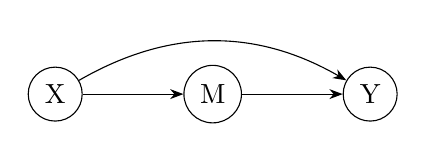
\begin{tikzpicture}[>=Stealth, node distance=2cm, on grid, auto]

        % Nodes
        \node (X) [draw, circle] {X};
        \node (M) [draw, circle, right=of X] {M};
        \node (Y) [draw, circle, right=of M] {Y};
      
        % Arrows
        \draw[->] (X) -- (M);
        \draw[->] (M) -- (Y);
        \draw[->] (X) to[bend left] (Y);
      
      \end{tikzpicture}
      \caption{Causal diagram showing $M$ mediating the effect of $X$ on $Y$.}    
      \label{fig:simp_med}
\end{figure}

We define the counterfactual $Y_x$ as the value $Y$ would assume when $X=x$. Similarly, write $M_x$ for the value $M$ would assume when $X=x$. Next, write $Y_{x,m}$ for the value $Y$ would assume if $X$ and $M$ were set to $x$ and $m$ respectively. Combining these ideas, we get the ``nested counterfactual'' $Y_{x, M_{x'}}$, which is the value of $Y$ when $X=x$ and $M$ is set to whatever it would have been when $X=x'$. It is common to link ordinary and nested conterfactuals by making the consistency assumption, which states $Y_x = Y_{x, M_x}$. Note that if $x \neq x'$ then the nested counterfactual is necessarily unobservable. It is nevertheless possible, given certain assumptions, to estimate the expected values of ordinary and nested counterfactuals. We will return later to the identification of expected counterfactuals with estimable quantities \hl{(I'm not certain whether it's better to do identification here or later).}

We now move on to the definition of various mediation effects which are of interest throughout the literature. There are three main types of mediation effect: total, direct and indirect, although the scale on which these are measured can vary. In the interest of generality, we write $d(y_1, y_2)$ for an arbitrary measure of the discrepancy between $y_1$ and $y_2$. The most natural form is $d(y_1, y_2) = y_1 - y_2$, although others may be more appropriate depending on context. Note that we do not require $d$ to be symmetric; in fact, the sign of $d$ is often of central scientific importance.

Proceeding now to the actual definitions, we define the total effect of $X$ on $Y$ to be $TE(x, x') = d(EY_x, EY_{x'})$. The direct effect is defined as $DE(x, x') = d(Y_{x, M_{x'}}, Y_{x', M_{x'}})$, and the indirect effect is $IE(x, x') = d(Y_{x, M_{x}}, Y_{x, M_{x'}})$. See, e.g., ??? for motivation and discussion of these definitions \hl{($g$-function?)}.

When the outcome, $Y$, is continuous, it is natural to take the discrepancy function to be $d(y_1, y_2) = y_1 - y_2$ as mentioned above. However, when $Y$ is binary, it is less obvious which scale to use. In this setting, expected counterfactuals are probabilities, so mediation effects measure the discrepancy between two probabilities. One option is to use the same difference preferred for continuous outcome; we refer to this as the risk-difference scale. Alternatives include $d(y_1, y_2) = y_1 / y_2$, the risk-ratio scale, and $d(y_1, y_2) = [y_1 / (1 - y_1)] / [y_2 / (1 - y_2)]$, the odds-ratio scale. We focus only on the binary outcome setting, although our results are easily extended to handle continuous outcomes. While our method can handle any choice of discrepancy function $d$ \hl{(differentiable? Whatever is necessary to apply the $\delta$-method later; might need to be continuously differentiable)}, in the interest of accessibility we specialize our results to the three discrepancies just mentioned for binary outcomes.



\subsection{Identification and Modelling of Expected Counterfactuals}

A fundamental problem of causal inference is that we can only ever observe one counterfactual outcome on a particular individual. In mediation analysis, this problem is even worse, since many of our definitions involve the nested counterfactual, $Y_{x, M_{x'}}$, which when $x \neq x'$ cannot be observed on any individual. Nevertheless, \citet{Ima10I} give conditions under which the population average of a nested counterfactual can be expressed in terms of conditional expectations, possibly conditional on one or more additional covariates, $W$. Specifically, their Theorem 1 states that, under a condition they call ``Sequential Ignorability'', we can write
%
\begin{equation}
    \bE (Y_{x, M_{x'}} | W=w) = \bE_M \left[ \bE_Y \left( Y | X=x, M, W=w \right) | X=x', W=w \right]. \label{eq:ID}
\end{equation}
%
In fact, their Theorem 1 is somewhat more general, giving an expression for the density of the nested counterfactual rather than its expected value.

Using Equation (\ref{eq:ID}), we can estimate expected nested counterfactuals by working with the more tractable conditional expectations of $Y$ and $M$. We model the latter using regression, either linear or logistic depending on the forms of $Y$ and $M$. If $Y$ and $M$ are binary, then Equation (\ref{eq:ID}) has a particularly simple form:
%
\begin{multline}
    \bE (Y_{x, M_{x'}} | W=w) = \bP \left( Y=1 | X=x, M=1, W=w \right) \bP(M=1 | X = x', W=w) \\ + \bP \left( Y=1 | X=x, M=0, W=w \right) \bP(M=0 | X = x', W=w). \label{eq:ID_bin}
\end{multline}
%
We estimate the conditional probabilities on the right-hand side of Equation (\ref{eq:ID_bin}) using logistic regression in the usual way. Note that this requires us to fit two models, one to predict $M$ using $X$ and $W$, while the other predicts $Y$ using $M$, $X$ and $W$.

We extend this regression modelling with the introduction of random effects \citep[see, e.g.][]{Dem04}. Specifically, we include random effects for the intercept and $X$ in our model for $M$, and for the intercept, $M$ and $X$ in our model for $Y$. We model these random effects as normally distributed, allowing for correlation within a model, but independent across models. Let $U \sim N(0, \Gamma_Y)$ and $V \sim N(0, \Gamma_M)$ be the random effects in our models for $Y$ and $M$ respectively. We can now re-write Equation (\ref{eq:ID_bin}) as
%
\begin{align}
    \bE (Y_{x, M_{x'}} | W=w) = & \left[\bE_U \bP \left( Y=1 |U, X=x, M=1, W=w \right) \right. \cdot \label{eq:ID_bin_ran}\\
    &  \left. \bE_V \bP(M=1 |V, X = x', W=w)\right] + \nonumber \\ 
    & \left[ \bE_U \bP \left( Y=1 |U, X=x, M=0, W=w \right) \right. \cdot \nonumber \\
    & \left. \bE_V \bP(M=0 |V, X = x', W=w) \right]. \nonumber 
\end{align}
%








%! START HERE



\textcolor{red}{The following discussion is awkward. I want to present a general expression for $E_U P(Y | ...)$, then specialize to Equation (\ref{eq:ID_bin_ran}). I have defined too much notation, but for now I'm just going to focus on getting ideas down on the page. Later, I will edit and tighten-up the presentation.}


We show an expansion for one term in Equation (\ref{eq:ID_bin_ran}); the rest follow similarly. First, write $\eta = (\beta_0 + \beta_X x + \beta_M m + B_W^T w) + (U_0 + U_X x + U_M m)$ for the linear predictor of $Y$ based on $X$, $M$ and $W$. Let $\mu = \beta_0 + \beta_X x + \beta_M m + B_W^T w$ be the fixed-effects component of $\eta$, and $\xi = U_0 + U_X x + U_M m$ be its random-effects component. For convenience, we will also write $\gamma^2_Y(c_1, c_2, c_3) = (c_1, c_2, c_3) \Gamma_Y (c_1, c_2, c_3)^T$, so that $\bV \xi = \gamma^2_Y(1, m, x)$.

It is a well-known fact about logistic regression that
%
\begin{equation}
    \bP \left( Y=1 |U, X=x, M=1, W=w \right) = \left[1 + \exp(-\eta)\right]^{-1},
\end{equation}
%
so the first term in Equation (\ref{eq:ID_bin_ran}) can be written as
%
\begin{align}
    \bE_U \bP \left( Y=1 |U, X=x, M=1, W=w \right) & = \int \frac{\phi_3(u; 0, \Gamma_Y)}{1 + \exp(-\eta)} du, \label{eq:pY1_bad}
\end{align}
%
where $\phi_d$ is the $d$-variate normal density. A straightforward change of variables gives us the alternative expression
%
\begin{align}
    \bE_U \bP \left( Y=1 |U, X=x, M=1, W=w \right) & = \int \frac{\phi_1(z; 0, 1)}{1 + \exp(-\mu - \gamma_Y(1, m, x) z)} dz. \label{eq:pY1}
\end{align}
%
Importantly, the integral in Equation (\ref{eq:pY1}) is univariate (and thus amenable to numerical evaluation using quadrature), while the integral in Equation (\ref{eq:pY1_bad}) is multivariate.

The integral in Equation (\ref{eq:pY1}) arises often enough that we give it a name. Let
%
\begin{equation}
    \Psi(\mu, \sigma^2) = \int \frac{\phi(z; 0, 1)}{1 + \exp(-\mu - \sigma z)} dz.
\end{equation}


\subsection{Old}


In this section, we define the total, direct and indirect mediation effects in terms of nested counterfactuals. We begin by applying the Mediation Formula of \citet{Pea12} to identify nested counterfactuals with simple functions of conditional expectations.

We begin by observing that mediation effects are often defined in terms of nested counterfactuals (regardless of the scale on which these effects are reported). \hl{There is some causal inference theory to be done here. For now, I'm just going to write what I expect to be true, then later I will go back and add the necessary assumptions.} As such, we begin by identifying a general nested counterfactual with estimable quantities. To this end, write $Y(x, m)$ for the counterfactual value of $Y$ when $X$ and $M$ are set to $x$ and $m$ respectively. Similarly, write $M(x)$ for the counterfactual value of $M$ when $X=x$. We write $Y(x, M(x'))$ for the value of $Y$ when $X$ is set to $x$ and $M$ is set to what it would have been if $X$ were $x'$. We refer to $Y(x, M(x'))$ as a nested counterfactual. Note that, when $x \neq x'$, the nested counterfactual is necessarily unobservable. Nevertheless, given regularity conditions, we can write
%
\begin{equation}
    \bE Y(x, M(x')) = \int \bE(Y | M=m, X=x) \bP(M = dm | X = x') \label{eq:id_nest}
\end{equation}
%
A similar expression holds conditional on pre-treatment covariates,
\begin{equation}
    \bE Y_c(x, M(x')) = \int \bE(Y | M=m, X=x, C=c) \bP(M = dm | X = x', C=c) \label{eq:id_nest_cov}
\end{equation}
%
Having identified expected nested counterfactuals with integrals of conditional quantities, we can use regression to estimate the RHS of Equations \ref{eq:id_nest} and \ref{eq:id_nest_cov}. This identification with regression-based quantities is especially simple if $M$ is binary. Here, we get $\bP(M=m | \cdot) = \bE(M=m | \cdot)$, where the latter quantity is popularly modelled with logistic regression. For simplicity, we hereafter assume that the mediator, $M$, is binary. \hl{If not, we need to do something different. One option is to extract the conditional density of $(M | \cdot)$, then perform the integral. Another is to do regression with response $\bE(Y | M=m, X=x, C=c)$, viewed as a function of $m$. There is likely an equivalence between these two methods; I can come back to this later.}

The above development allows only fixed-effects in the regression models. If we want to also incorporate random effects, we simply view Equations \ref{eq:id_nest} and \ref{eq:id_nest_cov} as having had these random effects marginalized out. That is, if we write $U$ and $V$ for the random effects in our models for $Y$ and $M$ respectively, and $G_V$, $G_V$ for the random effects' distributions, then we can re-write Equations \ref{eq:id_nest} and \ref{eq:id_nest_cov} as
%
\begin{align}
    \bE Y(x, M(x')) &= \int \bE(Y | U=u, M=m, X=x) \bP(M = dm |V=v, X = x') G_U(du) G_V(dv) \label{eq:ran_id_nest} \\
    \bE Y_c(x, M(x')) &= \int \bE(Y | U=u, M=m, X=x, C=c) \bP(M = dm | V=v, X = x', C=c) G_U(du) G_V(dv) \label{eq:ran_id_nest_cov}
\end{align}

\subsection{Ideas for CI Theory}
Applying the Counterfactual Unnesting Theorem of \citet{Cor21}, and provided that the conditions specified therein are satisfied, we have

Alternatively, see Theorem 1 of \citet{Ima10I}. This is specifically the result I want, not the corresponding identification results of \citet{Ima10II}, which focuses more narrowly on identification of mediation effects. Note that, in \citet{Ima10I}, the function $f$ is a density (with respect to some unspecified measure, possibly counting measure). In order to get the above formulas for expected values of $Y$, we do need to assume that $\bE Y$ is finite so we can apply Fubini's Theorem (the one for finite integrals).






\section{Estimation and Inference}

\begin{outline}
    \1 Estimate models using \texttt{lme4}
    \1 UQ for model parameters (mention \texttt{merDeriv} package)
    \1 UQ for nested counterfactuals via $\delta$-method
    \1 Simultaneous UQ for triples of mediation effects (i.e. total, direct and indirect)
        \2 Can also do all 9 simultaneously
    \1 UQ for predicted group-level effects?
\end{outline}


\section{Empirical Investigation}

\begin{outline}
    \1 Monte Carlo study
        \2 Proof of concept
        \2 Explore robustness. See \citet{Sam23} for inspiration.
    \1 Real data
        \2 Trust study dataset?
\end{outline}

\bibliography{../Bib-Exact_Asymptotics}

\end{document}